%Master File:lectures.tex


\lesson{Generative Models}
\vspace{-1cm}
\begin{center}
  \includegraphics[width=\linewidth]{GMplateLDA}
\end{center}
\keywords{Generative models, graphical models, LDA}
%%%%%%%%%%%%%%%%%%%%%%% Next Slide %%%%%%%%%%%%%%%%%%%%%%%
\renewcommand{\Outline}{%
\begin{slide}
\section[1]{Outline}

\begin{minipage}{10cm}\raggedright
  \begin{enumerate}\squeeze
    \outlineitem{Building Probabilistic Models}{generativemodel}
    \outlineitem{Graphical Models}{graphicalmodel}
    \outlineitem{Latent Dirichlet Allocation}{lda}
  \end{enumerate}
\end{minipage}\hfill
\begin{minipage}{12cm}
  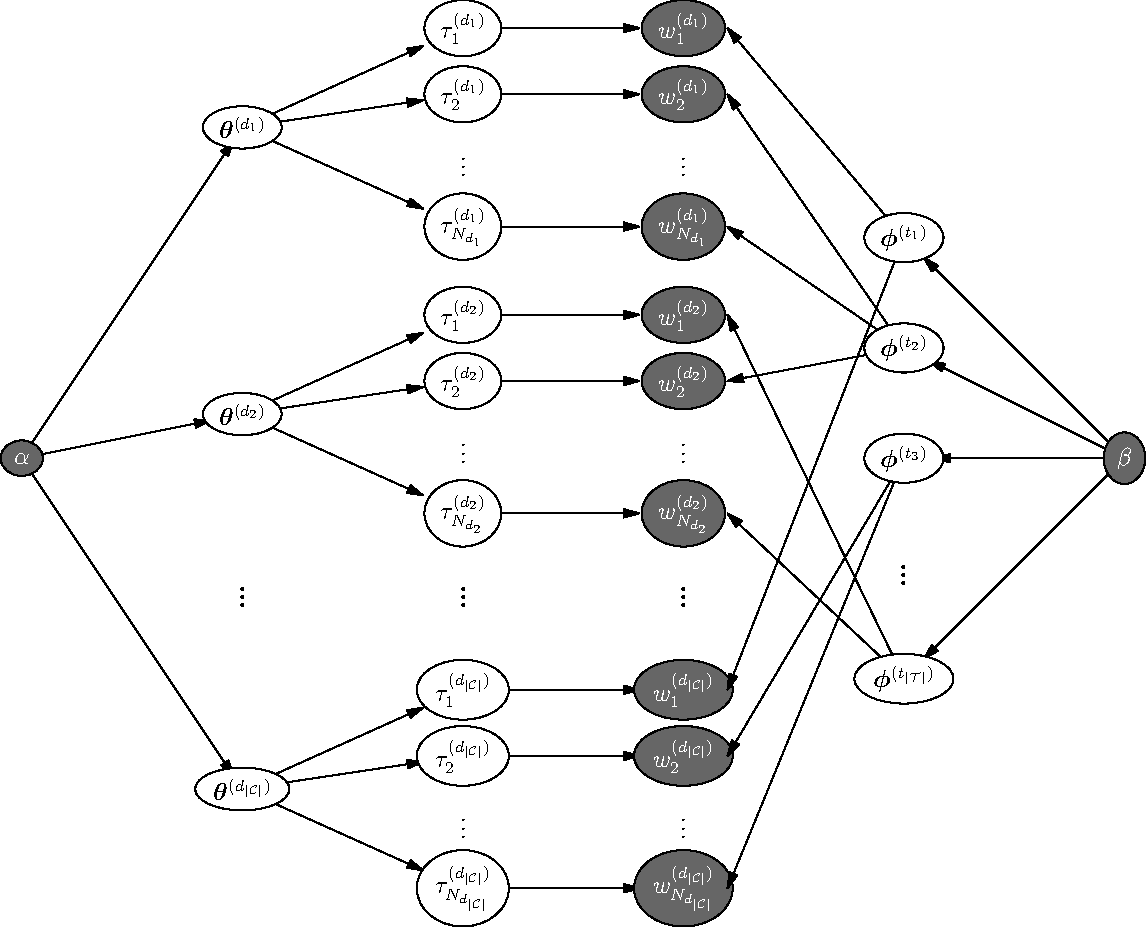
\includegraphics[width=12cm]{LDAGM}
\end{minipage}
\end{slide}
\addtocounter{outlineitem}{1}
}

\setcounter{outlineitem}{1}
\Outline % Motivation
\toptarget{firstoutline}
%%%%%%%%%%%%%%%%%%%%%%% Next Slide %%%%%%%%%%%%%%%%%%%%%%%

\begin{slide}
\section{Building Probabilistic Models}

\begin{PauseHighLight}
  \begin{itemize}
  \item To describe a system with uncertainty we use random variables,
    $X$, $Y$, $Z$, etc.\pause
  \item We use the convention of writing random variables in capitals
    (this is sometimes confusing as when you observe a random variables
    it is no longer random)\pause
  \item The variables are described by probability mass function
    $\Prob{X,Y,Z}$ or if our variables are continuous, but probability
    densities $f_{X,Y,Z}(x,y,z)$\pause
  \item We build in dependencies in this joint distribution\pause
  \end{itemize}
\end{PauseHighLight}

\end{slide}

%%%%%%%%%%%%%%%%%%%%%%% Next Slide %%%%%%%%%%%%%%%%%%%%%%%

\begin{slide}
\section{Discriminative Models}

\begin{PauseHighLight}
  \begin{itemize}
  \item We often think of our observations as given and the predictions
    as random variables\pause
  \item For example we might be given some features $\bm{x}$ and we wish
    to predict a class $C\in\mathcal{C}$\pause
  \item Our objective is then to find the probability $\Prob{C|\bm{x}}$\pause
  \item This is known as a \emph{discriminative model}\pause
  \item E.g.{} in \textit{foundations of machine learning} you learnt how to
    find the Bayes' optimal discrimination surface\pause
  \end{itemize}
\end{PauseHighLight}

\end{slide}


%%%%%%%%%%%%%%%%%%%%%%% Next Slide %%%%%%%%%%%%%%%%%%%%%%%

\begin{slide}
\section{Generative Models}

\begin{PauseHighLight}
  \begin{itemize}
  \item Sometimes it is easy to think about the joint process of
    generating the features and outputs together\pause
  \item This leads to a joint distribution $\Prob{\bm{X},Y}$ where
    $\bm{X}$ are your features and $Y$ is your output you are trying to
    predict\pause
  \item This is known as a \emph{generative model}\pause
  \item Generative models are often more natural to think about\pause
  \item We can use them to do discrimination using
    \begin{align*}
      \Prob{Y|\bm{X}} = \frac{\Prob{\bm{X},Y}}{\Prob{\bm{X}}}
      = \frac{\Prob{\bm{X},Y}}{\sum\limits_Y \Prob{\bm{X}, Y}}\pause
    \end{align*}
  \end{itemize}
\end{PauseHighLight}

\end{slide}

%%%%%%%%%%%%%%%%%%%%%%% Next Slide %%%%%%%%%%%%%%%%%%%%%%%

\begin{slide}
\section{Latent Variables}

\begin{PauseHighLight}
  \begin{itemize}
  \item Sometimes we have models that involve random variables that we
    don't observe and we don't care about\pause
  \item These are called \emph{latent variables}\pause
  \item If we have a latent variable $Z$ and observed variable $\bm{X}$
    and we are predicting a variable $Y$ then we would
    \emph{marginalise} over the latent variable
    \begin{align*}
      \Prob{\bm{X}, Y} = \sum_Z \Prob{\bm{X}, Y, Z}\pause
    \end{align*}
  \end{itemize}
\end{PauseHighLight}

\end{slide}

%%%%%%%%%%%%%%%%%%%%%%% Next Slide %%%%%%%%%%%%%%%%%%%%%%%

\begin{slide}
\section{Mixture of Gaussians}

\begin{PauseHighLight}
  \begin{itemize}
  \item Suppose we were observing the decays from two types of
    short-lived particle\pause
  \item We observe the half life, $X$, but not the particle type\pause
  \item We assume $X$ is normally distributed with unknown means and
    variances: $\bm{\Theta} = \{\mu_1$, $\sigma_1^2$, $\mu_2$,
    $\sigma_2^2\}$\pause
  \item Let $Z\in\{0,1\}$ be an indicator that it is particle 1\pause
  \item The probability of $X$ is given by
    \begin{align*}
      f(X|Z,\bm{\Theta}) = Z\,\normal{X\big|\mu_1,\sigma_1^2} +
      (1-Z)\,\normal{X\big|\mu_2,\sigma_2^2}\pause
    \end{align*}
  \end{itemize}
\end{PauseHighLight}

\end{slide}

%%%%%%%%%%%%%%%%%%%%%%% Next Slide %%%%%%%%%%%%%%%%%%%%%%%

\begin{slide}
\section[-2]{Data}

\begin{PauseHighLight}
  \begin{itemize}
  \item Note that
    \begin{align*}
      f(X|\bm{\Theta}) &= \sum_{Z\in\{0,1\}} f(X,Z|\bm{\Theta})\pause 
                         = \sum_{Z\in\{0,1\}}
      f(X|Z,\bm{\Theta})\,\Prob{Z}\pause \\ &= \av[Z]{f(X|Z,\bm{\Theta})}\pause
      = p \, \normal{X\big|\mu_1,\sigma_1^2} +
      (1-p)\,\normal{X\big|\mu_2,\sigma_2^2}\pause
    \end{align*}
  \end{itemize}
  \begin{center}
    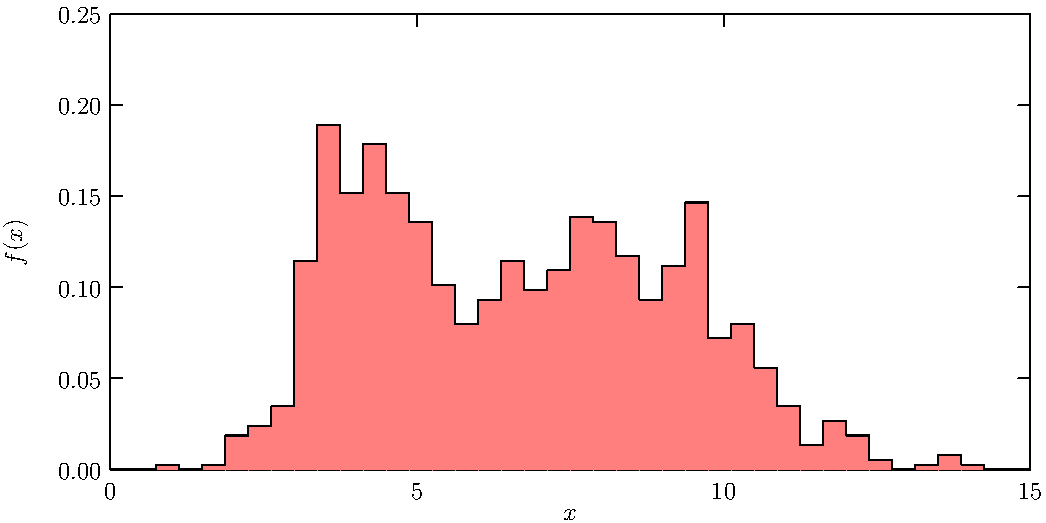
\includegraphics[width=0.8\linewidth]{mixtureOfGaussiansData}\pause
  \end{center}
\end{PauseHighLight}

\end{slide}

%%%%%%%%%%%%%%%%%%%%%%% Next Slide %%%%%%%%%%%%%%%%%%%%%%%

\begin{slide}
\section[-1]{Maximum Likelihood}

\begin{PauseHighLight}
  \begin{itemize}
  \item To solve the model as a Bayesian we would have to assign priors
    to our parameters $\bm{\Theta} = (\mu_1, \sigma_1, \mu_2,
    \sigma_2, p)$\pause
  \item This is doable, but complicated (we would also end up with a
    distribution for our parameters)\pause
  \item Often we only want a reasonable estimate for some of our
    parameters (e.g. the half-lives $\mu_1$ and $\mu_2$)\pause
  \item A reasonable approach is to seek those parameters that maximise the
    likelihood of our observed data
    \begin{align*}
      f(\data|\bm{\Theta}) = \prod_{X\in\data} f(X|\bm{\Theta})\pause
    \end{align*}
  \end{itemize}
\end{PauseHighLight}

\end{slide}

%%%%%%%%%%%%%%%%%%%%%%% Next Slide %%%%%%%%%%%%%%%%%%%%%%%

\begin{slide}
\section[-1]{EM Algorithm}

\begin{PauseHighLight}
  \begin{itemize}
  \item The maximum likelihood is a non-linear function of the
    parameters so cannot be immediately maximised\pause
  \item We have a difficulty in that our latent variable $Z$ will depend
    on the parameter $\bm{\Theta}$\pause
  \item And our likelihood will depend on the latent variable\pause
  \item We therefore proceed iteratively by maximising the expected
    log-likelihood with respect to the current set of parameters
    \begin{align*}
      \Theta^{(t+1)} = \mathop{\mathrm{argmax}}_{\bm{\Theta}}
      \sum_{\bm{Z}} \Prob{\bm{Z},\data|\bm{\Theta}^{(t)}}\,
      \logg{f(\data|\bm{Z}, \bm{\Theta})}\pause
    \end{align*}
  \item This is known as the \emph{expectation maximisation algorithm}\pause
  \end{itemize}
\end{PauseHighLight}

\end{slide}

%%%%%%%%%%%%%%%%%%%%%%% Next Slide %%%%%%%%%%%%%%%%%%%%%%%

\begin{slide}
\section{EM for Mixture of Gaussians}

\begin{PauseHighLight}
  \begin{itemize}
  \item Maximise with respect to parameters $\bm{\theta}$
    {\small
      \begin{align*}
      Q(\bm{\theta}|\bm{\theta}^{(t)})
      &= \sum_{\bm{Z}} \Prob{\bm{Z}|\data,\bm{\Theta}^{(t)}}\,
        \logg{f(\data|\bm{Z}, \bm{\Theta})} \\
      &=\sum_{i=1}^n \sum_{Z_i\in\{1,2\}} \Prob{Z_i|X_i,\bm{\theta}_i}\,
        \biggl( Z_i \log(p) + (1-Z_i)\log(1-p) \\
        & \hspace{9cm}  +
        \frac{(X_i-\mu_{Z_i})^2}{2\,\sigma^2_{Z_i}} - \logg{\sqrt{2\,\pi}\,\sigma_{Z_i}} \biggr)\pause
    \end{align*} }
  \item Compute update equations
    \begin{align*}
      \pd{Q(\bm{\theta}|\bm{\theta}^{(t)})}{\mu_k}=0,
      &&
         \pd{Q(\bm{\theta}|\bm{\theta}^{(t)})}{\sigma_k}=0,
      &&
          \pd{Q(\bm{\theta}|\bm{\theta}^{(t)})}{p}=0\pause
    \end{align*}
  \end{itemize}
\end{PauseHighLight}

\end{slide}

%%%%%%%%%%%%%%%%%%%%%%% Next Slide %%%%%%%%%%%%%%%%%%%%%%%

\begin{slide}
\section[-2]{Update Equations}

\begin{PauseHighLight}
  \begin{itemize}
  \item Means
    \begin{align*}
      \mu_{Z_i}^{(t+1)}
      &= \frac{ \sum_{i=1}^n \Prob{Z_i|X_i,\bm{\theta}^{(t)}} X_i}
        {\sum_{i=1}^n \Prob{Z_i|X_i,\bm{\theta}^{(t)}}},\pause
    \end{align*}
\item Variances
  \begin{align*}
    (\sigma_{Z_i}^{(t+1)})^2
      &= \frac{ \sum_{i=1}^n \Prob{Z_i|X_i,\bm{\theta}^{(t)}}
        (X_i-\mu^{(t+1)}_{Z_i})^2}
        {\sum_{i=1}^n \Prob{Z_i|X_i,\bm{\theta}^{(t)}}}\pause
  \end{align*}
  \item Probability of being type 1
    \begin{align*}
      p^{(t+1)} = \frac{1}{n} \sum_{i=1}^n \Prob{Z_i|X_i, \bm{\theta}_i}\pause
    \end{align*}
  \end{itemize}
\end{PauseHighLight}
  
\end{slide}


%%%%%%%%%%%%%%%%%%%%%%% Next Slide %%%%%%%%%%%%%%%%%%%%%%%

\begin{slide}
\section{Example}
\pause
\pb
\begin{center}
  \multipdf[width=\linewidth]{mixtureOfGaussians}\pause
\end{center}
\end{slide}

%%%%%%%%%%%%%%%%%%%%%%% Next Slide %%%%%%%%%%%%%%%%%%%%%%%
\Outline % Graphical Models
%%%%%%%%%%%%%%%%%%%%%%% Next Slide %%%%%%%%%%%%%%%%%%%%%%%

\begin{slide}
\section{Dependencies Between Variables}

\begin{PauseHighLight}
  \begin{itemize}
  \item In building a probabilistic model we want to know which random
    variables depend on each other directly and which don't\pause
  \item Variables that don't will typically still be correlated\pause
  \item If two random variables $X$ and $Y$ are correlated then
    \begin{itemize}
    \item $X$ could affect $Y$
    \item $Y$ could affect $X$
    \item $X$ and $Y$ could not influence each other, but both be
      affected by another random variable $Z$\pause
    \end{itemize}
  \end{itemize}
\end{PauseHighLight}

\end{slide}

%%%%%%%%%%%%%%%%%%%%%%% Next Slide %%%%%%%%%%%%%%%%%%%%%%%

\begin{slide}
\section{Graphical Models}

\begin{PauseHighLight}
  \begin{itemize}
  \item Graphical models are directed graphs that show causal
    relationships between random variables\pause
  \item We could represent the three conditions described above by
    \begin{center}
      \includegraphics[width=0.4\linewidth]{simpleGraphicalModels}\pause
    \end{center}
  \item We can use these graphical representations to work out how to
    efficiently average over latent variables\pause
  \end{itemize}
\end{PauseHighLight}

\end{slide}

%%%%%%%%%%%%%%%%%%%%%%% Next Slide %%%%%%%%%%%%%%%%%%%%%%%

\begin{slide}
\section{Statistical Independence}

\begin{PauseHighLight}
  \begin{itemize}
  \item Two random variables are statistically independent if
    \begin{align*}
      \Prob{X,Y} = \Prob{X} \, \Prob{Y}\pause
    \end{align*}
  \item Equally this implies $\Prob{X|Y} = \Prob{X}$ and $\Prob{Y|X} =
    \Prob{Y}$\pause
  \item Statistically independent variables are uncorrelated\pause
  \item But statistical independence is often too powerful\pause
  \end{itemize}
\end{PauseHighLight}

\end{slide}

%%%%%%%%%%%%%%%%%%%%%%% Next Slide %%%%%%%%%%%%%%%%%%%%%%%

\begin{slide}
\section[-1]{Conditional Independence}

\begin{PauseHighLight}
  \begin{itemize}
  \item A weaker notion is conditional independence
    \begin{minipage}{0.68\linewidth}
      \begin{align*}
        \Prob{X,Y|Z} = \Prob{X|Z} \, \Prob{Y|Z}\pause
      \end{align*}
    \end{minipage}\hfil
    \begin{minipage}{0.18\linewidth}
      \begin{center}
        \includegraphics[width=\linewidth]{conditionalIndependence}
      \end{center}
    \end{minipage}
  \item Conditional independence implies that there is no direct
    causation\pause
  \item But it doesn't imply zero correlation\pause
  \item Conditional independence reduces computational complexity, e.g.
    {\small \begin{align*}
      \av{X\,Y} = \sum_{X,Y,Z} X\,Y \, \Prob{X, Y, Z} \pause
      = \sum_Z P(Z) \left(\sum_X X P(X|Z) \right)  \left(\sum_Y Y P(Y|Z)
      \right)\pause
    \end{align*}}
  \end{itemize}
\end{PauseHighLight}

\end{slide}

%%%%%%%%%%%%%%%%%%%%%%% Next Slide %%%%%%%%%%%%%%%%%%%%%%%

\begin{slide}
\section{Graphical Models}

\begin{PauseHighLight}
  \begin{itemize}
  \item Graphical models often provide a quick way to represent the
    world\pause
    \begin{center}
      \includegraphics[width=\linewidth]{faultGP}
    \end{center}
  \item In graphical models we shade nodes that we observe\pause
  \item Note that the top events are conditionally independent if we make
    no observation, but are dependent if we observe a warning
    light!\pause
  \end{itemize}
\end{PauseHighLight}

\end{slide}

%%%%%%%%%%%%%%%%%%%%%%% Next Slide %%%%%%%%%%%%%%%%%%%%%%%
\Outline % LDA
%%%%%%%%%%%%%%%%%%%%%%% Next Slide %%%%%%%%%%%%%%%%%%%%%%%

\begin{slide}
\section{Model for Documents}

\begin{PauseHighLight}
  \begin{itemize}
  \item We consider a model for the words in a set of documents (we
    ignore word order)\pause
  \item We consider a corpus $\mathcal{C} = \{d_i | i = 1,\, 2,\, \ldots
    |\mathcal{C}|\}$\pause
  \item With documents consisting of words
    \begin{align*}
      d = \left(w_1^{(d)},\, w_2^{(d)},\, \ldots,\, w_{N_d}^{(d)}\right)\pause
    \end{align*}
  \item We assume that there is a set of topics
    $\mathcal{T}=\{t_1,\,t_2,\,\ldots,\, t_{|\mathcal{T}|}\}$\pause
  \item We associate a probability, $\theta^{(d)}_t$, that a
    word in document $d$ relates to a topic $t$\pause
  \end{itemize}
\end{PauseHighLight}

\end{slide}

%%%%%%%%%%%%%%%%%%%%%%% Next Slide %%%%%%%%%%%%%%%%%%%%%%%

\begin{slide}
\section[-1]{Documents and Topic}
\begin{center}
  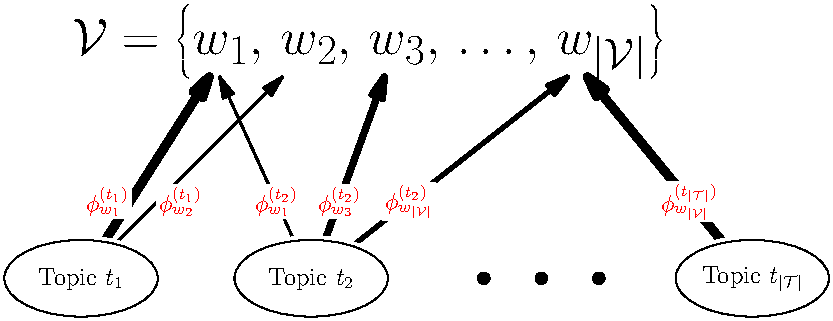
\includegraphics[width=\linewidth]{topicModel}\pause\\
  $\bm{\theta}^{(d)} = (\theta^{(d)}_t | t \in \mathcal{T})$\pause
\end{center}
\end{slide}

%%%%%%%%%%%%%%%%%%%%%%% Next Slide %%%%%%%%%%%%%%%%%%%%%%%

\begin{slide}
\section{Words and Topic}

\begin{PauseHighLight}
  \begin{itemize}
  \item We associate a probability $\phi^{(t)}_w$ that a word, $w$, is
    related to a topic $t$\pause
    \begin{center}
      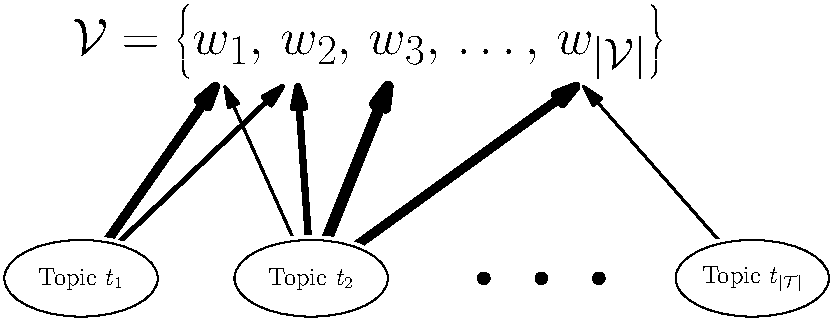
\includegraphics[width=0.7\linewidth]{topicModel1}\\\ \\
      $\bm{\phi}^{(t)} = (\phi^{(t)}_w | w \in \mathcal{V})$\pause
    \end{center}
  \end{itemize}
\end{PauseHighLight}

\end{slide}

%%%%%%%%%%%%%%%%%%%%%%% Next Slide %%%%%%%%%%%%%%%%%%%%%%%

\begin{slide}
\section[-2]{Dirichlet Allocation}

\begin{minipage}{0.5\linewidth}
  \begin{PauseHighLight}
  \begin{itemize}
  \item Most documents are predominantly about a few topics and most
    topic have a small number of words associated to them\pause
  \item We can generate sparse vectors $\bm{\theta}^{(d)}$ and
    $\bm{\phi}^{(t)}$ from a Dirichlet distribution with small parameters
    $\bm{\alpha}$ 
    \begin{align*}
      \mathrm{Dir}(\bm{p}|\bm{\alpha}) = \Gamma\!\left(\sum_i
      \alpha_i\right) \prod_{i=1}^n
      \frac{p_i^{\alpha_i-1}}{\Gamma(\alpha_i)}\pause
    \end{align*}
    \end{itemize}
\end{PauseHighLight}
\end{minipage}\hfil
\begin{minipage}{0.4\linewidth}
  \begin{center}
    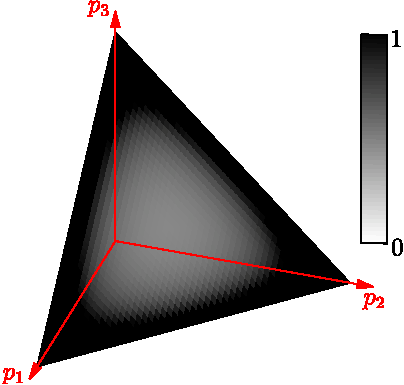
\includegraphics[width=0.95\linewidth]{dirichletSparse}\\
    $\bm{\theta}^{(d)} \sim \mathrm{Dir}(\alpha\,\bm{1})$\\
    $\bm{\phi}^{(t)}\sim \mathrm{Dir}(\beta\,\bm{1})$\pause
  \end{center}
\end{minipage}


\end{slide}

%%%%%%%%%%%%%%%%%%%%%%% Next Slide %%%%%%%%%%%%%%%%%%%%%%%

\begin{slide}
\section[-1]{Generating Document}

\begin{PauseHighLight}
  \begin{itemize}
  \item To generate a document we choose a topic for each word and a
    word for each topic\pause
    \begin{align*}
    \forall d\in\mathcal{C} \quad \bm{\theta}^{(d)}&\sim
    \mathrm{Dir}(\alpha\,\bm{1})\pause &&\\
    \forall t\in\mathcal{T} \quad \bm{\phi}^{(t)}&\sim
    \mathrm{Dir}(\beta\,\bm{1})\pause && \\
    \forall d\in\mathcal{C} \; \wedge\; \forall i\in\{1,\,2,\,\ldots, N_d\}
    \quad \tau^{(d)}_i &\sim \mathrm{Cat}(\bm{\theta}^{(d)}),\pause &
    w^{(d)}_i &\sim \mathrm{Cat}(\bm{\phi}^{(\tau^{(d)}_i)})
  \end{align*}
\item Where $\mathrm{Cat}(i|\bm{p}) = p_i$ is the categorical
  distribution (we choose one of a number of options)\pause
\item This model is known as \emph{Latent Dirichlet Allocation}\pause
  \end{itemize}
\end{PauseHighLight}

\end{slide}


%%%%%%%%%%%%%%%%%%%%%%% Next Slide %%%%%%%%%%%%%%%%%%%%%%%

\begin{slide}
\section[-2]{LDA Graphical Model (version 1)}

\begin{center}
  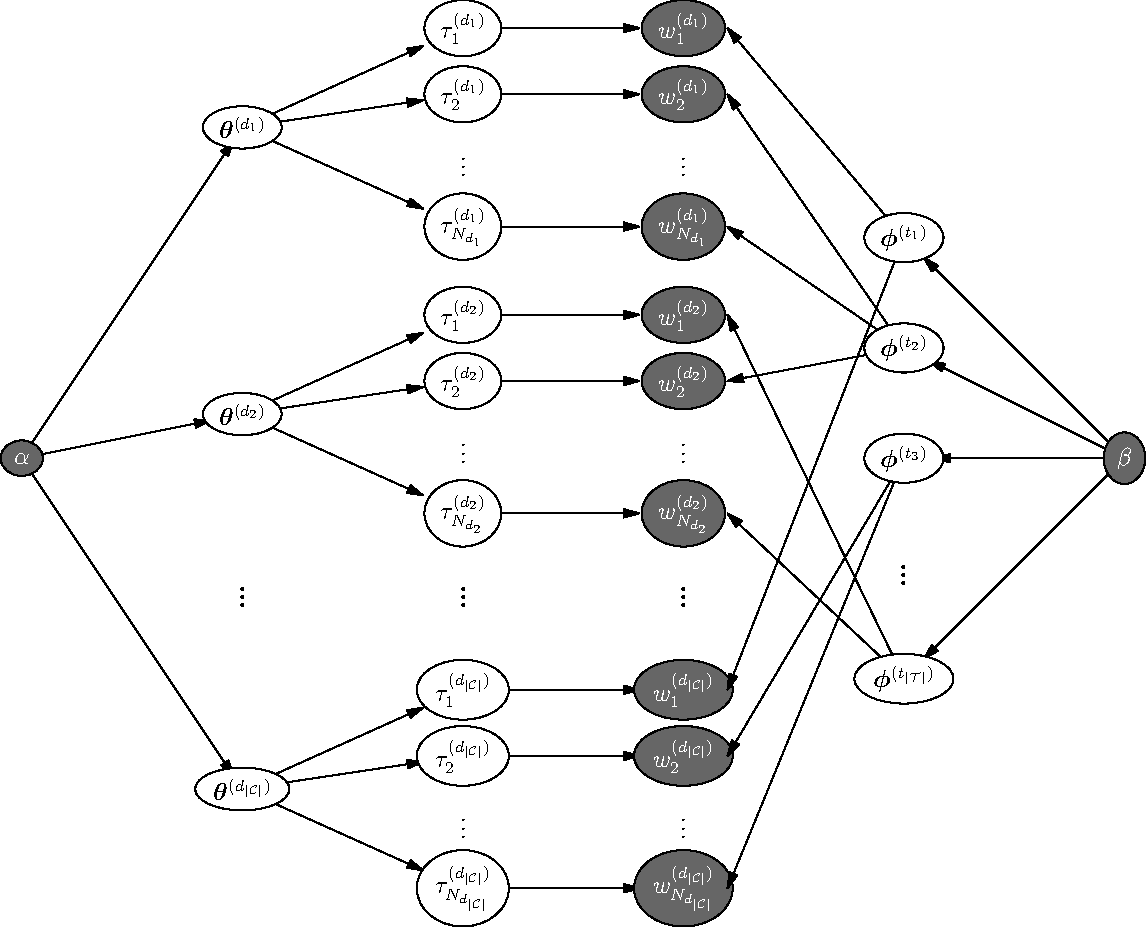
\includegraphics[width=0.8\linewidth]{LDAGM}
\end{center}
\end{slide}

%%%%%%%%%%%%%%%%%%%%%%% Next Slide %%%%%%%%%%%%%%%%%%%%%%%

\begin{slide}
\section{Plate Diagrams}

\begin{PauseHighLight}
  \begin{itemize}
  \item Drawing every random variable is tedious (and not really
    possible)\pause
  \item A short-hand is to draw a box (plate) meaning repeat
    \begin{center}
      \includegraphics[width=0.5\linewidth]{GMplateSimple}\pause
    \end{center}
  \item That is we generate vectors $\bm{\theta}^{d}$ from a Dirchelet
    distribution $\Dist[Dir]{\bm{\theta}|\alpha \bm{1}}$ for all
    documents in corpus $\mathcal{C}$\pause
  \end{itemize}
\end{PauseHighLight}

\end{slide}


%%%%%%%%%%%%%%%%%%%%%%% Next Slide %%%%%%%%%%%%%%%%%%%%%%%

\begin{slide}
\section{LDA Graphical Model (version 2)}

\begin{center}
  \includegraphics[width=\linewidth]{GMplateLDA}
\end{center}
\begin{PauseHighLight}
  \begin{itemize}
  \item This is a lot more compact\pause
  \item Personally, I find it hard to read, but you get used to it\pause
  \end{itemize}
\end{PauseHighLight}

\end{slide}

%%%%%%%%%%%%%%%%%%%%%%% Next Slide %%%%%%%%%%%%%%%%%%%%%%%

\begin{slide}
\section[-2]{Probabilistic Model}

\begin{PauseHighLight}
  \begin{itemize}
\item The graphical Model is shorthand for the variables
 {\small \begin{align*}
    \bm{W} &= (\bm{w}^{(d)} | d\in\mathcal{C})\quad \text{with} \quad
    \bm{w}^{(d)}=(w_1^{(d)},\, w_2^{(d)},\, \ldots,\, w_{N_d}^{(d)}),
    \quad \text{and}\quad w_i^{(d)} \in \mathcal{V} \\
    \bm{T} &= (\tau^{(d)}_i | d\in\mathcal{C}\;\wedge\;
    i\in\{1,\,2,\,\ldots, N_d\})\quad \text{with} \quad \tau^{(d)}_i \in
    \mathcal{T} \\
    \bm{\Theta} &=(\bm{\theta}^{(d)} | d\in\mathcal{C})\quad \text{with}
    \quad \bm{\theta}^{(d)} = (\theta^{(d)}_t | t \in \mathcal{T})\in
    \Lambda^{|\mathcal{T}|} \\
    \bm{\Phi} &= (\bm{\phi}^{(t)} | t \in \mathcal{T}) \quad \text{with}
    \quad \bm{\phi}^{(t)} = (\phi^{(t)}_w | w \in \mathcal{V}) \in
    \Lambda^{|\mathcal{V}|}\pause
  \end{align*}}
\item Distributed according to
  {\small\begin{align*}
    \Prob{\bm{W},\bm{T},\bm{\Theta},\bm{\Phi}\big|\alpha,\beta} =
    & \left(\prod_{t\in\mathcal{T}} \Dist[Dir]{\bm{\phi}^{(t)}\big|\beta\bm{1}}\right)
    \\ & \Biggl(\prod_{d\in\mathcal{C}} \Dist[Dir]{\bm{\theta}^{(d)}\big|\alpha\bm{1}}
     \prod_{i=1}^{N_d} \Dist[Cat]{\tau_i^{(d)}\big| \bm{\theta}^{(d)}}
    \Dist[Cat]{w_i^{(d)} \big| \bm{\phi}^{(\tau_i^{(d)})}}\Biggr)\pause
  \end{align*}}

\end{itemize}
\end{PauseHighLight}

\end{slide}

%%%%%%%%%%%%%%%%%%%%%%% Next Slide %%%%%%%%%%%%%%%%%%%%%%%

\begin{slide}
\section{Finding Topics}

\begin{PauseHighLight}
  \begin{itemize}
  \item We are given the set of words $\bm{W}$ and don't really care
    about $\tau_i^d$ the topic associated with word $i$ in document
    $d$\pause
  \item But we are interested in the words associated with each topic
    $\bm{\phi}^{(t_i)}$\pause
  \item And the topics associated with each document
    $\bm{\theta}^{(d)}$\pause
  \item To compute them we need to sample the probability
    distribution\pause
  \item One way to do this is using Monte Carlo methods (see next
    lecture)\pause 
  \end{itemize}
\end{PauseHighLight}

\end{slide}


%%%%%%%%%%%%%%%%%%%%%%% Next Slide %%%%%%%%%%%%%%%%%%%%%%%

\begin{slide}
\section{Summary}

\begin{PauseHighLight}
  \begin{itemize}
  \item Building probabilistic models is an intricate process\pause
  \item Identifying random variables that describe the system is the
    first step\pause
  \item Graphical models provides a representation showing the causal
    relationship between random variables\pause
  \item It is possible to generate very rich models such as Latent
    Dirchlet Allocation (LDA)\pause
  \end{itemize}
\end{PauseHighLight}

\end{slide}
